\begin{filecontents*}{hll_plot_data.csv}
n,uncorrected,hllpp,corrected,bits
1,0.0010,0.0489,0.0010,0.000
2,0.0010,0.0978,0.0010,0.000
3,0.0010,0.2762,0.0010,0.000
4,0.0010,0.2923,0.0010,0.000
5,0.0010,0.4746,0.0010,0.000
6,0.0010,0.6731,0.0010,0.000
7,0.0010,0.8247,0.0010,0.000
8,0.0010,0.8539,0.0010,0.000
9,0.0010,0.8889,0.0010,0.000
10,0.0010,0.9579,0.0010,0.000
11,0.0010,0.9883,0.0010,0.000
12,0.0010,0.9915,0.0010,0.000
13,0.0010,1.0518,0.0010,0.000
14,0.0010,1.1758,0.0010,0.000
15,0.0010,1.2201,0.0010,0.000
16,0.0010,1.2612,0.0010,0.000
17,0.0010,1.3731,0.0010,0.000
18,0.0010,1.4618,0.0010,0.000
19,0.0010,1.5471,0.0010,0.000
20,0.0010,1.5960,0.0010,0.000
21,0.0010,1.6203,0.0010,0.000
22,0.0010,1.6508,0.0010,0.000
23,0.0010,1.6587,0.0010,0.000
24,0.0010,1.6749,0.0010,0.000
25,0.0010,1.6971,0.0010,0.000
26,0.0010,1.7751,0.0010,0.000
27,0.0010,1.7847,0.0010,0.000
28,0.0010,1.8321,0.0010,0.000
29,0.0010,1.8817,0.0010,0.000
30,0.0010,1.9171,0.0010,0.000
31,0.0010,1.9140,0.0010,0.000
33,0.0010,1.9317,0.0010,0.000
35,0.0010,1.9192,0.0010,0.000
37,0.0010,1.8566,0.0010,0.000
39,0.0010,1.7873,0.0010,0.000
41,0.0010,1.7100,0.0010,0.000
44,0.0010,1.6119,0.0010,0.000
47,0.0010,1.6321,0.0010,0.000
50,0.0010,1.7757,0.0010,0.000
53,0.0010,1.8482,0.0010,24.000
56,0.0010,1.9385,0.0010,24.000
59,0.0010,1.9704,0.0010,24.000
62,0.0010,1.9331,0.0010,24.000
66,0.0010,1.8749,0.0010,24.000
70,0.0010,1.9091,0.0010,24.000
74,0.0010,1.8445,0.0010,24.000
78,0.0010,1.7200,0.0010,24.000
82,0.0010,1.6400,0.0010,24.000
87,0.0010,1.6858,0.0010,24.000
92,0.0010,1.6435,0.0010,24.000
97,0.0010,1.6939,0.0010,24.000
102,0.0010,1.7287,0.0010,24.000
108,0.0010,1.7121,0.0010,24.000
114,0.0010,1.7156,0.0010,24.000
120,0.0010,1.7565,0.0010,24.000
126,0.0010,1.7577,0.0010,24.000
133,0.0029,1.7483,0.0037,24.000
140,0.0028,1.6920,0.0036,24.000
147,0.0027,1.7551,0.0035,24.000
155,0.0025,1.6865,0.0034,24.000
163,0.0024,1.7946,0.0033,24.000
172,0.0023,1.8369,0.0033,24.000
181,0.0022,1.8620,0.0032,24.000
191,0.0020,1.8564,0.0032,24.000
201,0.0019,1.8950,0.0031,24.000
212,0.0018,1.8844,0.0031,24.000
223,0.0018,1.8612,0.0031,24.000
235,0.0033,1.8461,0.0047,24.000
247,0.0032,1.8938,0.0046,24.000
260,0.0090,1.8772,0.0119,23.000
273,0.0100,1.8761,0.0131,23.000
287,0.0095,1.8853,0.0127,23.000
302,0.0103,1.8310,0.0137,23.000
318,0.0111,1.8510,0.0145,23.000
334,0.0105,1.8587,0.0142,23.000
351,0.0145,1.7915,0.0219,22.000
369,0.0191,1.8355,0.0340,21.000
388,0.0292,1.8441,0.0549,20.234
408,0.0373,1.8404,0.0645,20.000
429,0.0865,1.9535,0.1184,19.000
451,0.1689,1.9757,0.1588,18.109
474,0.1813,1.9867,0.1539,18.000
498,0.3781,1.9825,0.7968,17.000
523,0.3906,1.9509,0.8029,17.000
550,8.2585,1.9729,1.0994,16.000
578,8.6539,2.0061,1.1019,16.000
607,9.0751,2.0254,1.0621,16.000
638,9.5109,2.0597,1.0911,16.000
670,9.9434,2.0951,1.0811,16.000
704,10.4170,2.1076,1.0525,16.000
740,10.9333,2.1297,1.0931,16.000
777,11.4468,2.1437,1.1061,16.000
816,11.9332,2.0844,1.0949,16.000
857,12.4613,2.1098,1.1147,16.000
900,13.0273,2.0712,1.0852,16.000
945,13.5599,2.0945,1.0540,16.000
993,14.1620,2.0847,1.0510,16.000
1043,14.7835,2.1334,1.0340,16.000
1096,15.4211,2.2927,1.0226,16.000
1151,16.0896,2.2596,0.9960,16.000
1209,16.7723,2.3258,0.9984,16.000
1270,17.5120,2.3477,1.0191,16.000
1334,18.2560,2.4093,1.0039,16.000
1401,19.0246,2.4053,1.0119,16.000
1472,19.8080,2.4435,1.0186,16.000
1546,20.6038,2.4106,1.0263,16.000
1624,21.4413,2.4928,1.0684,16.000
1706,22.3226,2.5174,1.0819,16.000
1792,23.2232,2.5474,1.1092,16.000
1882,24.0946,2.4984,1.1630,16.000
1977,25.0215,2.4492,1.1429,16.000
2076,26.0110,2.4562,1.1069,16.000
2180,27.5786,2.0106,1.3293,16.000
2289,29.7510,4.1259,3.5757,16.000
\end{filecontents*}
\begin{filecontents*}{hll_timing.csv}
n,hybrid_ins,dense_ins,hybrid_est,dense_est
165,1229.87,15.21,13009.31,718.19
231,415.53,15.66,7297.07,718.00
323,1862.62,15.31,8713.79,718.99
453,2204.95,15.69,14192.30,719.12
634,1743.95,15.34,11771.13,718.60
888,2209.93,15.24,12248.65,718.81
1244,2960.74,15.63,16866.59,718.85
1742,3902.05,15.66,17276.01,719.08
2439,15.66,15.24,738.91,719.98
3415,15.59,16.22,740.53,720.80
4781,15.67,15.60,739.26,719.57
6693,15.79,15.59,739.25,718.62
9370,15.71,15.57,723.92,700.69
13119,16.05,15.27,721.16,699.47
18366,15.65,15.30,720.31,700.02
25713,16.13,15.67,720.34,699.47
35999,15.61,15.24,721.48,698.48
50398,15.62,15.24,721.18,698.40
70558,16.03,16.31,720.65,698.07
98781,15.64,15.27,719.83,699.44
\end{filecontents*}
\documentclass[11pt,a4paper]{article}
\usepackage[margin=1.6cm]{geometry}
\usepackage{amsmath,amssymb,graphicx}
\usepackage{pgfplots}
\pgfplotsset{compat=1.16}
\usetikzlibrary{positioning}
\usepackage{algpseudocode}
\pagestyle{empty}
\begin{document}
\begin{center}\large\textbf{Hash-list cardinality correction (table-free occupancy inverse)}\end{center}

\medskip
\noindent\textbf{Setting.} We want the number of distinct items $n$ in a large stream while storing far less memory than the items themselves. This is cardinality estimation, and HyperLogLog (HLL) is the standard tool. It hashes each item and keeps an array of $m=2^{P}$ small counters called registers, and from their distribution it estimates $n$ with a relative error of about $1.04/\sqrt{m}$ regardless of $n$. That array is the dense representation.

\noindent While the set is small this implementation is more accurate than registers, because it keeps the items explicitly in two compact stages before falling back to registers. First a value list, the exact sorted list of inserted values, so the count is exact. Then a hash list, a compact sorted list of the distinct hashes of the items. Only when the hash list no longer fits does the counter convert to dense registers. This note is about the estimator for the hash-list stage.

\noindent In the hash list each item is reduced to a composite hash, a $w$-bit fingerprint built from the register-bucket index ($P$ bits), the item's leading-zero count, and a few residual bits. The list keeps the distinct composites sorted, and to stay compact it stores only the gap from each composite to the next, Rice-coded (a variable-length encoding cheap for small integers, with a per-cell optimal parameter). Sorting is what makes those gaps small. Their number $D$ is what we observe. While $w$ is large, distinct items almost never share a composite, so $D$ equals the true count $n$. To pack more items as the list fills, the counter shrinks $w$, and then two distinct items can collide onto the same composite, so $D$ starts to undercount $n$. The correction below recovers $n$ from the observed $D$ and the current width $w$.

\medskip
\noindent\textbf{What a hash-list entry is.} A stored composite is a $w$-bit string. The top $P$ bits are the register-bucket index, and the tail ($t=w-P$ bits) holds the register (the leading-zero count, what dense HLL keeps) plus extra resolution that is kept while $w$ is wide. The tail takes three forms.

\begin{center}
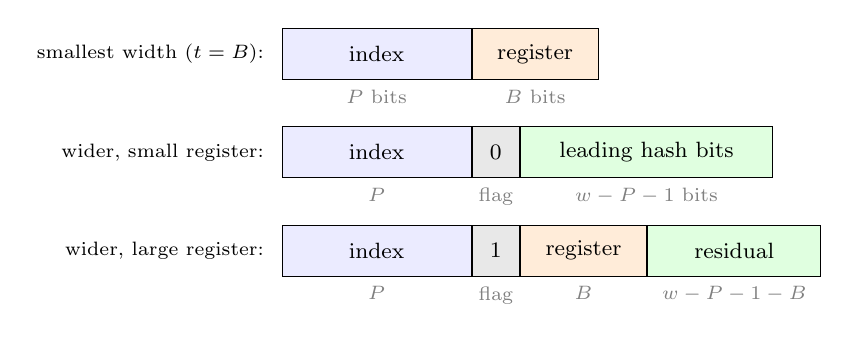
\begin{tikzpicture}[font=\footnotesize,
  b/.style={draw, minimum height=6.5mm, anchor=west, inner xsep=3pt},
  rl/.style={anchor=east, font=\scriptsize},
  bl/.style={anchor=north, font=\scriptsize, text=gray}]
\node[rl] at (-1mm,0) {smallest width ($t=B$):};
\node[b, fill=blue!8, minimum width=24mm] (a) at (0,0) {index};
\node[b, fill=orange!15, minimum width=16mm, right=0pt of a] (bb) {register};
\node[bl] at (a.south) {$P$ bits};
\node[bl] at (bb.south) {$B$ bits};
\node[rl] at (-1mm,-1.25) {wider, small register:};
\node[b, fill=blue!8, minimum width=24mm] (c) at (0,-1.25) {index};
\node[b, fill=gray!18, minimum width=6mm, right=0pt of c] (d) {0};
\node[b, fill=green!12, minimum width=32mm, right=0pt of d] (e) {leading hash bits};
\node[bl] at (c.south) {$P$};
\node[bl] at (d.south) {flag};
\node[bl] at (e.south) {$w-P-1$ bits};
\node[rl] at (-1mm,-2.5) {wider, large register:};
\node[b, fill=blue!8, minimum width=24mm] (f) at (0,-2.5) {index};
\node[b, fill=gray!18, minimum width=6mm, right=0pt of f] (g) {1};
\node[b, fill=orange!15, minimum width=16mm, right=0pt of g] (h) {register};
\node[b, fill=green!12, minimum width=22mm, right=0pt of h] (k) {residual};
\node[bl] at (f.south) {$P$};
\node[bl] at (g.south) {flag};
\node[bl] at (h.south) {$B$};
\node[bl] at (k.south) {$w-P-1-B$};
\end{tikzpicture}
\end{center}
\noindent The index selects the bucket and the register is what dense HLL would store. The leading bits or residual are the extra resolution the counter drops as it shrinks $w$ to pack more entries, which is what lets distinct items collide. The diagram is one composite's logical layout. On disk the entries are sorted and each is stored as the Rice-coded gap to the previous one, not in full.

\medskip
\noindent\textbf{Notation.} Precision $P$ (so $m=2^{P}$ registers), bits per register $B$, current composite width $w$, tail $t=w-P$, observed distinct composites $D$, and largest storable register value $R=2^{B}-1$.

\medskip
\noindent Write $g(n):=\mathbb{E}[D\mid n,w]$ for the expected distinct-composite count at cardinality $n$. The estimate $\hat{n}$ is the cardinality whose expected count matches the observed $D$, that is, $g$ inverted at $D$ (computed by safeguarded Newton iteration\footnote{Newton's method solves $g(n)=D$ by repeatedly jumping to where the tangent of $g$ meets $D$: from a guess it moves to $n-(g(n)-D)/g'(n)$. That is fast but can overshoot or run away when the curve is flat. The safeguard keeps an interval $[\mathrm{low},\mathrm{high}]$ known to contain the answer (here $\mathrm{low}=D$, with $\mathrm{high}$ doubled until $g(\mathrm{high})\ge D$) and takes the Newton jump only when it lands inside that interval, otherwise it halves the interval instead (bisection). Halving is slow but always shrinks the interval and never leaves it, so the method always reaches the answer.}):
\begin{equation}\label{eq:est}
\mathbb{E}[D\mid \hat{n},w]=D,
\qquad\text{equivalently}\qquad
\hat{n}=g^{-1}(D).
\end{equation}
Equation \eqref{eq:occ} counts how many distinct composite values get used. Picture each possible composite as a box and each of the $n$ items as landing in the box named by its composite. Two items in the same box collide, so the number of non-empty boxes (the distinct count $D$) falls below $n$, the same effect as shared birthdays in a room. The expected number of non-empty boxes, summed over groups of $g_j$ equally likely boxes of probability $p_j$, is \eqref{eq:occ}, and its derivative \eqref{eq:deriv} drives the Newton step:
\begin{align}
\mathbb{E}[D\mid n,w]&\;=\;\sum_{j} \underbrace{g_j}_{\substack{\text{cells in}\\\text{group }j}}\,\underbrace{\Bigl(1-(1-p_j)^{\,n}\Bigr)}_{\Pr[\text{cell occupied by }n\text{ elements}]}, \label{eq:occ}\\[2pt]
\frac{\partial}{\partial n}\mathbb{E}[D\mid n,w]&\;=\;\sum_{j} g_j\,\underbrace{\bigl(-\ln(1-p_j)\bigr)}_{>0}\,(1-p_j)^{\,n}. \label{eq:deriv}
\end{align}
The cell groups follow from the composite encoding (uniform $P$-bit index, geometric register, uniform residual). At the smallest width $t=B$ the tail is just the register, giving \eqref{eq:small}. At wider widths a flag bit selects between storing the leading hash bits or the register plus a residual, giving \eqref{eq:wide}:
\begin{equation}\label{eq:small}
\mathbb{E}[D\mid n]
=2^{P}\Bigl[\;
\underbrace{\sum_{r=1}^{R-1}\bigl(1-(1-2^{-(P+r)})^{n}\bigr)}_{\text{geometric registers }r=1,\dots,R-1}
\;+\;
\underbrace{\bigl(1-(1-2^{-(P+R-1)})^{n}\bigr)}_{\text{saturating register}}
\;\Bigr].
\end{equation}
\begin{equation}\label{eq:wide}
\resizebox{\linewidth}{!}{$\displaystyle
\mathbb{E}[D\mid n,w]
=2^{P}\Bigl[
\underbrace{\sum_{\ell=0}^{\min(B,\,t-2)} 2^{\,t-2-\ell}\bigl(1-(1-2^{-(w-1)})^{n}\bigr)}_{\text{flag }0:\ r\le B+1,\ \text{leading bits stored}}
+
\underbrace{\sum_{r=B+2}^{R-1} 2^{\,t-1-B}\bigl(1-(1-2^{-(P+r+t-1-B)})^{n}\bigr)}_{\text{flag }1:\ \text{register}+\text{residual}}
+
\underbrace{2^{\,t-1-B}\bigl(1-(1-2^{-(P+R-1+t-1-B)})^{n}\bigr)}_{\text{saturating register}}
\Bigr]$}.
\end{equation}

\medskip
\noindent\textbf{The estimator in pseudocode.} The uncorrected estimate is just the stored distinct count. The corrected estimate inverts \eqref{eq:occ} for $n$.
\begin{algorithmic}[1]
\Function{Uncorrected}{}
  \State \Return $D$ \Comment{$D$ is the number of distinct composites stored}
\EndFunction
\Statex
\Function{Corrected}{$D,\,w$} \Comment{$w$ is the current width, $P$ and $B$ fixed}
  \State $E(n) \gets \sum_{(g,p)} g\,\bigl(1-(1-p)^{n}\bigr)$ \Comment{cell groups $(g,p)$ of eq.\ (4)/(5)}
  \State $E'(n) \gets \sum_{(g,p)} g\,\bigl(-\ln(1-p)\bigr)(1-p)^{n}$
  \State $low \gets D,\quad high \gets D$
  \While{$E(high) < D$} \Comment{grow until the root is bracketed}
    \State $high \gets 2\,high$
  \EndWhile
  \State $n \gets (low+high)/2$
  \Repeat
    \If{$E(n) > D$}
      \State $high \gets n$
    \Else
      \State $low \gets n$
    \EndIf
    \State $candidate \gets n - (E(n)-D)/E'(n)$ \Comment{Newton step}
    \If{$low < candidate < high$}
      \State $n_{\mathrm{next}} \gets candidate$
    \Else
      \State $n_{\mathrm{next}} \gets (low+high)/2$ \Comment{bisection fallback}
    \EndIf
    \State $\delta \gets \lvert n_{\mathrm{next}} - n\rvert$
    \State $n \gets n_{\mathrm{next}}$
  \Until{$\delta \le 10^{-12}\,n$} \Comment{relative step below $10^{-12}$}
  \State \Return $n$
\EndFunction
\end{algorithmic}

\medskip
\noindent\textbf{Complexity.} \textsc{Uncorrected} is $O(1)$: the distinct count $D$ is maintained in the counter's metadata and read directly, not recomputed by scanning the stored entries. \textsc{Corrected} is $O(2^{B})$ per estimate: $E$ and $E'$ each sum over the $O(2^{B})$ cell groups, and the safeguarded Newton loop runs a bounded number of iterations (plus $O(\log(n/D))$ steps to grow the bracket). It depends on neither the cardinality $n$ nor the register count $m=2^{P}$, and never scans the stored entries. Each cell group evaluates a logarithm and an exponential, so its constant is larger than the dense estimate's $O(m)$ register scan, which is why the estimate-timing figure shows it slower in absolute terms despite touching fewer items. A hash-list insert, by contrast, splices into the sorted buffer and is $O(D)$ in the worst case, so its cost grows as the list fills, while a register insert is $O(1)$.

\medskip
\noindent Accuracy at $P=10,\ B=6$: mean absolute relative error over 256 seeds (one seed cannot rank unbiased estimators, only the spread over seeds can). The uncorrected count $D$ is biased low and worsens toward conversion. HLL++ (the dense estimate of the same elements) is unbiased but carries the full $1.04/\sqrt{m}$ register noise. The occupancy inverse \eqref{eq:est} stays below both. The dotted curve (right axis) is the average composite width, which falls from 24 to 16 bits ($=P+B$) as the list fills, and each narrowing raises the collision rate that drives the uncorrected error up. Dashed verticals: value list ends at $n=52$, registers begin near $n=2153$.

\begin{center}
\begin{tikzpicture}
\begin{axis}[
  name=erraxis, width=15cm, height=5.2cm, scale only axis,
  axis y line*=left,
  xlabel={true cardinality $n$}, ylabel={mean abs.\ relative error (\%)},
  xmin=0, xmax=2300, ymode=log, ymin=0.001, ymax=40,
  legend cell align=left, legend columns=2,
  legend style={font=\small, at={(0.5,-0.30)}, anchor=north,
    /tikz/every even column/.append style={column sep=0.5cm}},
  grid=both, grid style={gray!20},
  tick label style={font=\small}, label style={font=\small},
]
\draw[gray, densely dashed] (axis cs:52,0.001) -- (axis cs:52,40);
\draw[gray, densely dashed] (axis cs:2153,0.001) -- (axis cs:2153,40);
\node[gray, font=\scriptsize, rotate=90, anchor=south] at (axis cs:52,0.09) {value list ends};
\node[gray, font=\scriptsize, rotate=90, anchor=south] at (axis cs:2153,0.09) {registers begin};
\addplot[red, thick] table[col sep=comma, x=n, y=uncorrected] {hll_plot_data.csv};
\addlegendentry{uncorrected (stored distinct count $D$)}
\addplot[orange, thick] table[col sep=comma, x=n, y=hllpp] {hll_plot_data.csv};
\addlegendentry{HLL++ (dense registers)}
\addplot[blue, thick] table[col sep=comma, x=n, y=corrected] {hll_plot_data.csv};
\addlegendentry{corrected (occupancy inverse, eq.~\ref{eq:est})}
\addlegendimage{black, densely dotted, thick}
\addlegendentry{avg composite width (right axis)}
\end{axis}
\begin{axis}[
  width=15cm, height=5.2cm, scale only axis,
  axis y line*=right, axis x line=none,
  xmin=0, xmax=2300, ymin=14, ymax=26,
  ylabel={avg composite width (bits)},
  tick label style={font=\small}, label style={font=\small},
]
\addplot[black, densely dotted, thick, restrict y to domain=1:100,
  unbounded coords=discard]
  table[col sep=comma, x=n, y=bits] {hll_plot_data.csv};
\end{axis}
\end{tikzpicture}
\end{center}

\medskip
\noindent Aggregate errors over the hash-list range (256 seeds, $P=10,\ B=6$): MAE is the mean absolute error in elements, MRE the mean (signed) relative error, MSE the mean squared error in elements$^2$.
\begin{center}
\begin{tabular}{lrrr}
\hline
estimator & MAE (elements) & MRE & MSE (elements$^2$)\\
\hline
uncorrected ($D$)            & $208.9$ & $-14.00\%$ & $76286$\\
HLL++ (dense registers)      & $25.9$  & $-0.01\%$  & $1398$\\
corrected (occupancy inverse)& $11.5$  & $-0.05\%$  & $297$\\
\hline
\end{tabular}
\end{center}
\noindent The corrected estimate is about $2.3\times$ better than HLL++ on MAE and $4.7\times$ on MSE, both are unbiased (MRE near zero), while the uncorrected count is biased low by $14\%$.

\medskip
\noindent That accuracy is not free: the hybrid pays a much higher per-insert cost in the hash list than the dense registers. Mean per-insert time (200 reps, log-log): in the hash list each insert splices into a sorted gap-coded buffer at roughly 1 to 4 microseconds, about 80 to 250 times the $\sim 16$ ns register insert, until conversion near $n=2153$ collapses it to register speed.
\begin{center}
\begin{tikzpicture}
\begin{axis}[
  width=15cm, height=4.6cm, scale only axis,
  xlabel={true cardinality $n$}, ylabel={ns per insert},
  xmode=log, ymode=log, xmin=120, xmax=130000, ymin=8, ymax=6000,
  legend cell align=left, legend pos=north east, legend style={font=\small},
  grid=both, grid style={gray!20},
  tick label style={font=\small}, label style={font=\small},
]
\draw[gray, densely dashed] (axis cs:2153,8) -- (axis cs:2153,6000);
\node[gray, font=\scriptsize, rotate=90, anchor=south] at (axis cs:2153,30) {registers begin};
\addplot[blue, thick, mark=*, mark size=1pt] table[col sep=comma, x=n, y=hybrid_ins] {hll_timing.csv};
\addlegendentry{hybrid (hash list, then registers)}
\addplot[orange, thick, mark=*, mark size=1pt] table[col sep=comma, x=n, y=dense_ins] {hll_timing.csv};
\addlegendentry{HLL++ (registers only)}
\end{axis}
\end{tikzpicture}
\end{center}

\medskip
\noindent The same trade-off appears when estimating: the table-free occupancy inversion (a Newton solve over the cell groups) costs more per query than the dense estimate, about 7 to 17 microseconds in the hash list versus $\sim 0.7$ microseconds, again collapsing to dense cost after conversion. This is per query, not per element, so it matters far less than the insert cost.
\begin{center}
\begin{tikzpicture}
\begin{axis}[
  width=15cm, height=4.6cm, scale only axis,
  xlabel={true cardinality $n$}, ylabel={ns per estimate},
  xmode=log, ymode=log, xmin=120, xmax=130000, ymin=300, ymax=30000,
  legend cell align=left, legend pos=north east, legend style={font=\small},
  grid=both, grid style={gray!20},
  tick label style={font=\small}, label style={font=\small},
]
\draw[gray, densely dashed] (axis cs:2153,300) -- (axis cs:2153,30000);
\node[gray, font=\scriptsize, rotate=90, anchor=south] at (axis cs:2153,1100) {registers begin};
\addplot[blue, thick, mark=*, mark size=1pt] table[col sep=comma, x=n, y=hybrid_est] {hll_timing.csv};
\addlegendentry{hybrid (occupancy inverse, then dense)}
\addplot[orange, thick, mark=*, mark size=1pt] table[col sep=comma, x=n, y=dense_est] {hll_timing.csv};
\addlegendentry{HLL++ (dense estimate)}
\end{axis}
\end{tikzpicture}
\end{center}

\medskip
{\small
\noindent\textbf{Why no table.} The correction is derived analytically from the encoding, under HyperLogLog's usual uniform-hash assumption, so it stores nothing. A calibrated per-cell table fed the observed duplicate count would lower variance, but only by 5 to 18 percent in the tail, inside the $1.04/\sqrt{m}$ floor we already clear, and it costs about 38 KB of coefficients (roughly 1600 lines, 72 breakpoints per cell over 45 cells) regenerated by a multi-hour Monte Carlo per precision and bit-width set, plus insertion-order dependence. Table-free avoids all of it: nothing to fit or rerun, correct at every precision, never out of sync with the encoding, and path-independent.
}
\end{document}
